% Provenance (never printed): old premiere S material on plate kinematics (rigid
% plates, rates from magnetic anomalies and from satellite positioning, hotspots
% and the Hawaiian chain, the coherence of the model); see
% sources/book2/PROVENANCE.md. Velocities from the NNR-MORVEL56 poles
% (figdata/grade-11/plate_velocities.py), station series from the Nevada Geodetic
% Laboratory (gnss_series.py), volcano ages from Clague and Dalrymple 1987
% (hawaii_chain.py). Euler poles and triple junctions belong to Year 1: the
% rotation pole is told, not defined.
\chapter{Las placas y sus movimientos}\label{ch:g11:plate-motions}

Cerca de la cima del Mauna Kea, en la isla de Hawái, una antena fijada a la
roca recibe cada día, desde octubre de 1996, las señales de los satélites de
posicionamiento. Cada día un ordenador calcula dónde está la antena, con una
precisión de pocos milímetros. Treinta años de posiciones cuentan cada año la
misma historia: la antena, la montaña y la isla entera se desplazan unos
\qty{7}{cm} al año hacia el oeste-noroeste, sin detenerse y sin girar. En 2026
la antena estaba a más de dos metros de su punto de partida. Este capítulo
mide esos movimientos, muestra cómo encajan unos con otros sobre una esfera y
lee el mismo movimiento en la cadena de volcanes apagados que se extiende desde
Hawái a través del Pacífico norte.
% ledger: data:b2-ngl-gnss

\begin{recall}
La \omterm{def:g11:lithosphere-asthenosphere:lithosphere}{litosfera} está fragmentada en placas tectónicas que se mueven unas respecto
de otras a razón de pocos centímetros al año; sus límites son dorsales, fosas,
zonas de colisión y fallas transformantes (Libro 1, año 7). Un punto caliente
es un lugar del manto profundo que alimenta un volcán en la placa que tiene
encima; la placa se lleva el volcán mientras crece uno nuevo sobre el punto
caliente (Libro 1, año 7). Un receptor de posicionamiento por satélite
calcula su propia posición a partir de las señales de varios satélites
(Libro 1, año 9). Las bandas magnéticas del fondo oceánico dan la \omterm{def:g11:drift-to-spreading:spreading-rate}{velocidad de
expansión} de una dorsal (el \cref{ch:g11:drift-to-spreading}), y la \omterm{def:g11:lithosphere-asthenosphere:lithosphere}{litosfera}
es la capa externa rígida de la Tierra, de unos \qty{100}{km} de espesor
(el \cref{ch:g11:lithosphere-asthenosphere}). Una velocidad de \qty{1}{cm} al
año son \qty{10}{km} por millón de años, y \qty{1}{mm} al año es \qty{1}{km}
por millón de años.
\end{recall}

\begin{omfigure}
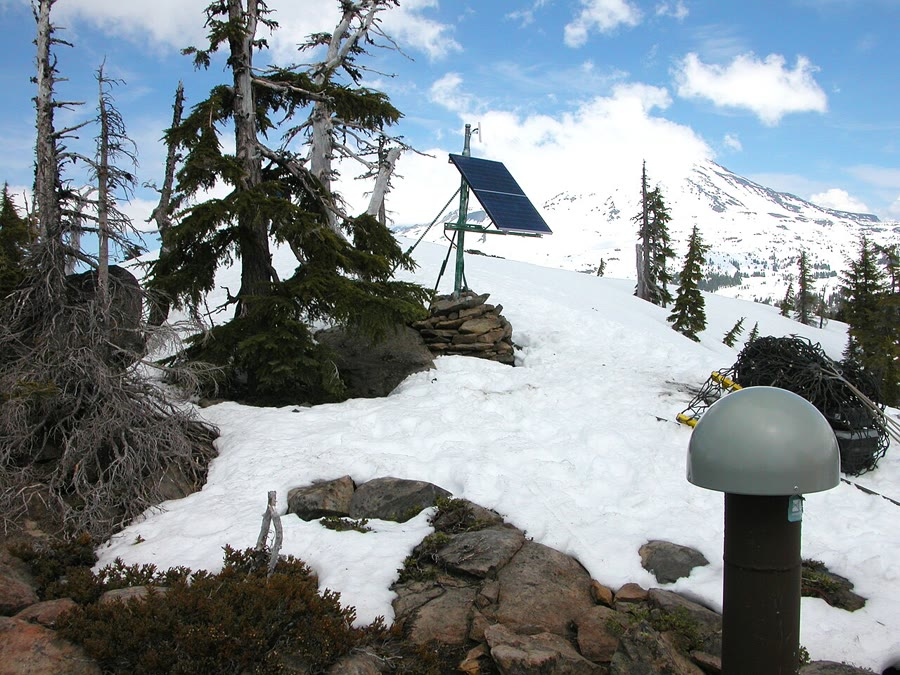
\includegraphics[width=0.62\linewidth]{images/book2/g11-usgs-gps-station.jpg}

{\small Una estación permanente de posicionamiento por satélite sobre un
volcán de la cordillera de las Cascadas, en Oregón (2007). La antena está bajo
la cúpula gris, en un mástil bien anclado en el suelo; el panel solar de detrás
alimenta el receptor. Una estación así registra su propia posición día tras
día. Fotografía: Dave Sherrod, USGS (dominio público).}
\end{omfigure}
% ledger: photo:g11-gps-station

\section{Placas rígidas sobre una esfera}

Los terremotos no están repartidos al azar por la Tierra: casi todos se
producen a lo largo de franjas estrechas, los límites de placas (Libro 1,
año 7). En el interior de una placa la roca apenas se rompe. Una placa no es,
por tanto, una piel blanda que se estira y se arruga al moverse, sino un trozo
rígido de \omterm{def:g11:lithosphere-asthenosphere:lithosphere}{litosfera} que se mueve en bloque.

\begin{definition}[Placa rígida]\label{def:g11:plate-motions:rigid-plate}
Una \emph{placa rígida}\index{placa rigida@placa rígida} es un trozo de \omterm{def:g11:lithosphere-asthenosphere:lithosphere}{litosfera} que se
mueve como un solo bloque: las distancias entre sus puntos no cambian, y su
deformación se concentra en zonas estrechas a lo largo de sus límites.
\end{definition}

El modelo de \omterm{def:g11:plate-motions:rigid-plate}{placas rígidas} es una aproximación. Algunas regiones se deforman
a lo largo de cientos de kilómetros, como las altas mesetas situadas tras el
Himalaya o el oeste de América del Norte, y el modelo las trata como límites
anchos. Pero en la mayor parte de la superficie de la Tierra funciona
notablemente bien: las velocidades que predice para las \omterm{def:g11:plate-motions:rigid-plate}{placas rígidas}
coinciden con las que miden las estaciones de satélite con un margen de pocos
milímetros al año (la \cref{sec:g11:plate-motions:predictive}), mientras que las
placas se mueven unas respecto de otras a razón de centímetros al año.

¿Cómo puede moverse un casquete rígido sobre la superficie de una esfera? No
puede deslizarse en línea recta, porque una recta se sale de la esfera. Sea
cual sea el movimiento de un casquete rígido, es una \emph{rotación} alrededor
de un eje que pasa por el centro de la Tierra. El eje corta la superficie en
el \emph{polo de rotación} de la placa. Un punto de la placa se mueve a lo
largo de un círculo menor alrededor de ese polo, y cuanto más lejos del polo
está, mayor es su círculo y más deprisa se mueve (figura siguiente). La
demostración de que todo movimiento de un casquete rígido es una rotación de
este tipo, y el uso de los polos de rotación para describir los límites de
placas, corresponden al Libro~3; aquí solo se usan las velocidades.

\begin{omfigure}
\begin{tikzpicture}[scale=1.15, font=\footnotesize]
  \fill[omSea!45] (0,0) circle (2);
  \draw (0,0) circle (2);
  % small circles about the rotation pole (pole at the top), seen slightly from above
  \foreach \a/\len in {60/0.75, 35/1.23, 0/1.5} {
    \pgfmathsetmacro{\r}{2*cos(\a)}
    \pgfmathsetmacro{\h}{2*sin(\a)}
    \draw[black!45, densely dashed] (-\r,\h) arc[start angle=180, end angle=0, x radius=\r, y radius=0.22*\r];
    \draw[omDef!80!black, line width=0.7pt] (-\r,\h) arc[start angle=180, end angle=360, x radius=\r, y radius=0.22*\r];
    \draw[-{Stealth[length=5pt]}, omProp, line width=1.1pt] (0,\h-0.22*\r) -- ++(\len,0);
  }
  \draw[black!70, dash pattern=on 3pt off 2pt] (0,-2.5) -- (0,2.55);
  \fill (0,2) circle (1.6pt);
  \node[anchor=south west] at (0.05,2.02) {polo de rotación};
  \node[anchor=north, text=black!70] at (0,-2.5) {eje de rotación, por el centro};
  \fill (0,0) circle (1pt);
  \node[anchor=west, align=left] at (2.25,0.9) {cada punto se mueve\\por un círculo menor\\alrededor del polo};
  \node[anchor=west, align=left, text=omProp] at (2.25,-0.4) {velocidad: máxima\\a \ang{90} del polo};
\end{tikzpicture}

{\small Una \omterm{def:g11:plate-motions:rigid-plate}{placa rígida} sobre una esfera gira alrededor de un eje que pasa por
el centro de la Tierra. Los puntos cercanos al polo de rotación se mueven
despacio, por círculos menores; los puntos situados a \ang{90} del polo son los
más rápidos (flechas: velocidades a escala).}
\end{omfigure}

La velocidad de un punto es fácil de calcular. Un punto a una distancia
angular $\theta$ del polo está a la distancia $R\sin\theta$ del eje, donde
$R = \qty{6371}{km}$ es el radio de la Tierra. Si la placa gira $\omega$
grados por millón de años, el punto recorre en un millón de años la fracción
$\omega/360$ del círculo de radio $R\sin\theta$:
\[
  v = \frac{\omega}{360} \times 2\pi R\sin\theta
    = \frac{\pi\,\omega}{180}\,R\sin\theta .
\]
Para $\omega = \qty{1}{\degree}$ por millón de años y $\theta = \ang{90}$
esto da $\pi \times 6371/180 \approx \qty{111}{km}$ por millón de años, es
decir, \qty{11.1}{cm} al año. Una placa no tiene, por tanto, una sola
velocidad: sus puntos se mueven a velocidades que van desde cero en el polo de
rotación (si el polo está en la placa) hasta un máximo a \ang{90} de él. Las
fallas transformantes de una dorsal, por las que dos placas se deslizan una
junto a otra, siguen círculos menores alrededor del polo de la rotación
relativa de las dos placas.
% ledger: earth:Rmean (shared), nnr56:poles

Los conjuntos publicados de polos de rotación dan, para cada placa, la
posición de su polo y su ritmo de giro. Uno de ellos, construido sobre todo a
partir de las velocidades y las direcciones de expansión medidas a lo largo de
las dorsales, describe 56 placas; la placa del Pacífico gira
\ang{0.651} por millón de años, la placa euroasiática \ang{0.223}. Con estos
números un ordenador calcula la velocidad de cualquier punto de cualquier
placa (mapa siguiente).
% ledger: nnr56:poles, nnr56:data

\begin{omfigure}
\begin{tikzpicture}
\begin{axis}[ommap, width=\linewidth, xtick={-180,-90,...,180}, ytick={-60,0,60}]
\addplot[fill=omLithAlluv, draw=black!45, line width=0.2pt] table {figdata/out/shared-geo-land.dat};
\addplot[omRidge, line width=0.6pt] table {figdata/out/shared-geo-school-ridge.dat};
\addplot[omRidge!70!black, line width=0.6pt] table {figdata/out/shared-geo-school-transform.dat};
\addplot[omTrench, line width=0.6pt] table {figdata/out/shared-geo-school-subduction.dat};
\addplot[fill=omTrench, draw=none] table {figdata/out/shared-geo-school-teeth.dat};
\addplot[black!65, line width=0.6pt] table {figdata/out/shared-geo-school-collision.dat};
% computed in figdata/grade-11/plate_velocities.py (NNR-MORVEL56); 2.5 degrees per cm/yr
\addplot[black, line width=0.8pt, -{Stealth[length=4pt]}, quiver={u=\thisrow{dx}, v=\thisrow{dy}}]
  table[x=lon, y=lat] {figdata/out/grade-11-plate_velocities-arrows.dat};
\addplot[omProp, line width=1.2pt, -{Stealth[length=5pt]}, quiver={u=\thisrow{dx}, v=\thisrow{dy}}]
  table[x=lon, y=lat] {figdata/out/grade-11-plate_velocities-hawaii.dat};
\addplot[only marks, mark=*, mark size=1.3pt, omProp] coordinates {(-155.46,19.80)};
\node[font=\scriptsize, anchor=north, fill=white, fill opacity=0.75, text opacity=1, inner sep=1pt]
  at (axis cs:-150,15) {Mauna Kea};
\draw[black, line width=0.8pt, -{Stealth[length=4pt]}] (axis cs:-172,-80) -- (axis cs:-147,-80);
\node[font=\scriptsize, anchor=west, fill=white, fill opacity=0.75, text opacity=1, inner sep=1pt]
  at (axis cs:-145,-80) {\qty{10}{cm} al año};
\end{axis}
\end{tikzpicture}

{\small Velocidades de puntos del interior de 16 placas, calculadas a partir
de sus polos de rotación publicados, en un marco en el que la \omterm{def:g11:lithosphere-asthenosphere:lithosphere}{litosfera} en su
conjunto no gira. Las placas del Pacífico, de Nazca, de Cocos, australiana e
india son las más rápidas; las placas euroasiática, norteamericana,
sudamericana y antártica, las más lentas. Flecha roja: la placa del Pacífico
en el Mauna Kea. Polos de rotación: Argus, Gordon y DeMets (2011); límites de
placas: Bird (2003); tierras emergidas: Natural Earth.}
\end{omfigure}
% ledger: nnr56:poles, data:pb2002, data:ne-land

\section{Medir los movimientos}

\subsection{Dos maneras de medir una velocidad}

Las bandas magnéticas del fondo oceánico dan la velocidad a la que dos placas
se separan a ambos lados de una dorsal (el \cref{ch:g11:drift-to-spreading}):
se divide la distancia de una banda al eje de la dorsal entre su edad. La
velocidad obtenida es una media sobre la edad de la banda, a menudo los
últimos millones de años, y es una velocidad \emph{relativa}, la de una placa
vista desde la otra. Las bandas no dicen nada de las placas que se encuentran
en una fosa o en una zona de colisión, porque allí no se forma fondo oceánico.

El posicionamiento por satélite mide el movimiento de un solo punto, hoy, a lo
largo de unos años o unas décadas. Una estación permanente está anclada a la
roca firme, de modo que se mueve con la placa; sus posiciones diarias,
representadas frente al tiempo, se alinean sobre una recta cuya pendiente es
la velocidad de la estación.

\begin{method}[Una velocidad a partir de una serie temporal de posiciones]\label{met:g11:plate-motions:rate}
\begin{enumerate}
  \item Representa la posición este y la posición norte de la estación frente
        al tiempo, en dos gráficas o en la misma.
  \item Traza la recta que mejor sigue cada serie (o lee dos puntos muy
        alejados de ella). Su pendiente, en milímetros al año, es la velocidad
        hacia el este $v_E$ o hacia el norte $v_N$; una estación que se mueve
        hacia el oeste o hacia el sur tiene una velocidad negativa.
  \item La velocidad de la estación es $v = \sqrt{v_E^2 + v_N^2}$; su
        dirección forma con la línea este--oeste el ángulo $\alpha$ tal que
        $\tan\alpha = |v_N|/|v_E|$, hacia el norte si $v_N > 0$ y hacia
        el este si $v_E > 0$.
\end{enumerate}
\end{method}

\begin{omfigure}
\begin{tikzpicture}
\begin{axis}[ompt, name=a, width=0.5\linewidth, height=5.6cm, xmin=1995, xmax=2027, ymin=-200, ymax=120,
  xlabel={año}, ylabel={posición (\unit{cm})}, xtick={2000,2010,2020},
  xticklabel style={/pgf/number format/set thousands separator={}},
  title={\small Mauna Kea, Hawái (MKEA)}, tick label style={font=\scriptsize}]
% computed in figdata/grade-11/gnss_series.py; ledger: data:b2-ngl-gnss
\addplot[only marks, mark=*, mark size=0.5pt, omDef] table[x=year, y=north] {figdata/out/grade-11-gnss_series-mkea.dat};
\addplot[only marks, mark=*, mark size=0.5pt, omProp] table[x=year, y=east] {figdata/out/grade-11-gnss_series-mkea.dat};
\node[font=\scriptsize, text=omDef!80!black, anchor=west] at (axis cs:1996.5,80) {norte};
\node[font=\scriptsize, text=omProp!80!black, anchor=west] at (axis cs:1996.5,-120) {este};
\end{axis}
\begin{axis}[ompt, at={(a.east)}, anchor=west, xshift=0.9cm, width=0.5\linewidth, height=5.6cm, xmin=1995, xmax=2027,
  ymin=-10, ymax=70, xlabel={año}, xtick={2000,2010,2020},
  xticklabel style={/pgf/number format/set thousands separator={}},
  title={\small Wettzell, Alemania (WTZR)}, tick label style={font=\scriptsize}]
\addplot[only marks, mark=*, mark size=0.5pt, omDef] table[x=year, y=north] {figdata/out/grade-11-gnss_series-wtzr.dat};
\addplot[only marks, mark=*, mark size=0.5pt, omProp] table[x=year, y=east] {figdata/out/grade-11-gnss_series-wtzr.dat};
\node[font=\scriptsize, text=omDef!80!black, anchor=west] at (axis cs:2014,22) {norte};
\node[font=\scriptsize, text=omProp!80!black, anchor=west] at (axis cs:2006,40) {este};
\end{axis}
\end{tikzpicture}

{\small Posiciones medias mensuales de dos estaciones permanentes, medidas
desde su primer mes: este (rojo) y norte (azul). Cada serie se alinea sobre
una recta, cuya pendiente es la velocidad de la estación en esa dirección. El Mauna Kea, en la placa del Pacífico, se mueve hacia el oeste y el norte; Wettzell, en
la placa euroasiática, hacia el este y el norte, unas tres veces más despacio.
Datos: Nevada Geodetic Laboratory (Blewitt, Hammond y Kreemer, 2018).}
\end{omfigure}
% ledger: data:b2-ngl-gnss

\begin{example}[La estación del Mauna Kea]\label{ex:g11:plate-motions:mkea}
De octubre de 1996 a septiembre de 2026, las posiciones mensuales de la
estación del Mauna Kea siguen dos rectas de pendientes $v_E =
\qty{-63.2}{mm}$ al año (hacia el oeste) y $v_N = \qty{+34.5}{mm}$ al año. La
velocidad es $\sqrt{63.2^2 + 34.5^2} \approx \qty{72}{mm}$ al año, y $\tan\alpha
= 34.5/63.2 \approx 0.546$ da $\alpha \approx \ang{29}$: la estación se mueve
\qty{7.2}{cm} al año en dirección oeste, desviada \ang{29} hacia el norte. El
polo de rotación de la placa del Pacífico predice en este lugar
\qty{6.9}{cm} al año, en dirección oeste desviada \ang{28} hacia el norte.
\end{example}
% ledger: data:b2-ngl-gnss, nnr56:poles (prediction computed in plate_velocities.py)

Los puntos se dispersan unos pocos milímetros alrededor de las rectas, mucho
menos que el movimiento de un solo año: tras unos años de medidas, la
velocidad de una estación se conoce con un margen mejor que un milímetro al año.

\subsection{Movimiento relativo y movimiento absoluto}

Una velocidad siempre se mide respecto de algo. La estación del Mauna Kea se
mueve \qty{7.2}{cm} al año respecto de un marco ligado a la Tierra entera;
vista desde una estación de América del Norte, que también se mueve, su
velocidad es otra.

\begin{definition}[Movimiento relativo; movimiento absoluto]\label{def:g11:plate-motions:relative-motion}
El \emph{movimiento relativo}\index{movimiento relativo} de una placa $A$
respecto de una placa $B$ es su movimiento tal como lo ve un observador
situado sobre $B$. El \emph{movimiento absoluto}\index{movimiento absoluto}
de una placa es su movimiento respecto de un marco ligado a la Tierra
profunda, por ejemplo un conjunto de puntos calientes que se suponen fijos, o
el marco en el que la \omterm{def:g11:lithosphere-asthenosphere:lithosphere}{litosfera} en su conjunto no gira.
\end{definition}

Las dorsales, las fosas y las fallas transformantes las modelan los
\omterm{def:g11:plate-motions:relative-motion}{movimientos relativos}: lo que importa en un límite es cómo se mueven las dos
placas una respecto de la otra. Las velocidades relativas se suman como los
desplazamientos que producen.

\begin{proposition}[Las velocidades relativas se suman como flechas]\label{prop:g11:plate-motions:sum}
Sea $\vec v_{A/B}$ la velocidad de la placa $A$ respecto de la placa $B$, en
un punto dado del límite, y lo mismo para los demás pares. Para tres placas
cualesquiera $A$, $B$, $C$,
\[
  \vec v_{A/C} = \vec v_{A/B} + \vec v_{B/C},
  \qquad\text{y}\qquad
  \vec v_{B/A} = -\vec v_{A/B}.
\]
\end{proposition}

\begin{proof}
En un tiempo corto $\Delta t$, sea un punto fijo de $A$ que pasa de la
posición $P$ a $P'$ visto desde $C$, y sea el punto de $B$ que estaba en $P$
y pasa a $Q$ visto desde $C$. Visto desde $B$, el punto de $A$ ha ido de $Q$
a $P'$. Los desplazamientos se suman como vectores:
$\overrightarrow{PP'} = \overrightarrow{PQ} + \overrightarrow{QP'}$, es decir,
desplazamiento de $A$ visto desde $C$ = desplazamiento de $B$ visto desde $C$
+ desplazamiento de $A$ visto desde $B$. Al dividir entre $\Delta t$ se
obtiene $\vec v_{A/C}
= \vec v_{B/C} + \vec v_{A/B}$. Con $C = A$, el primer miembro es nulo: $\vec
v_{B/A} = -\vec v_{A/B}$.
\end{proof}

\begin{method}[Cerrar un triángulo de velocidades]\label{met:g11:plate-motions:triangle}
\begin{enumerate}
  \item Escribe cada velocidad conocida con sus componentes este y norte,
        todas medidas en el mismo punto.
  \item Para hallar $\vec v_{A/B}$ a partir de las velocidades de $A$ y $B$ en
        el mismo marco $C$, resta: $\vec v_{A/B} = \vec v_{A/C} - \vec v_{B/C}$,
        componente a componente.
  \item En un dibujo, coloca los orígenes de $\vec v_{A/C}$ y $\vec v_{B/C}$
        en el mismo punto: la flecha que va del extremo de $\vec v_{B/C}$ al
        extremo de $\vec v_{A/C}$ es $\vec v_{A/B}$, y cierra el triángulo.
  \item Calcula su longitud y su dirección como en el
        \cref{met:g11:plate-motions:rate}.
\end{enumerate}
\end{method}

\begin{example}[La falla de San Andrés]\label{ex:g11:plate-motions:san-andreas}
En el centro de California, a \ang{35.5} N y \ang{120.5} O, los polos de
rotación dan a la placa del Pacífico la velocidad $(-42.1, +26.4)$ y a la
placa norteamericana $(-11.9, -14.8)$, en milímetros al año (este, norte), en
el marco de la \omterm{def:g11:lithosphere-asthenosphere:lithosphere}{litosfera} entera. La placa del Pacífico respecto de América del
Norte se mueve a $(-42.1 + 11.9,\ 26.4 + 14.8) = (-30.2, +41.2)$, es decir,
a $\sqrt{30.2^2 + 41.2^2} \approx \qty{51}{mm}$ al año, en dirección norte,
desviada \ang{36} hacia el oeste (figura siguiente). La falla de
San Andrés, que corre hacia el noroeste, absorbe la mayor parte de este
deslizamiento.
\end{example}
% ledger: nnr56:poles (computed in plate_velocities.py: relative pa/na at 120.5 W 35.5 N)

\begin{omfigure}
\begin{tikzpicture}[x=0.065cm, y=0.065cm, font=\footnotesize]
  % mm/yr, from plate_velocities.py: PA (-42.1, 26.4), NA (-11.9, -14.8), PA/NA (-30.2, 41.2)
  \draw[black!25] (-8,0) -- (8,0) (0,-8) -- (0,8);
  \draw[-{Stealth[length=5pt]}, omProp, line width=1.1pt] (0,0) -- (-42.1,26.4)
    node[pos=0.55, above right, inner sep=1pt] {$\vec v_{\mathrm{PA}}$};
  \draw[-{Stealth[length=5pt]}, omDef, line width=1.1pt] (0,0) -- (-11.9,-14.8)
    node[pos=0.8, right=2pt] {$\vec v_{\mathrm{NA}}$};
  \draw[-{Stealth[length=5pt]}, black, line width=1.1pt] (-11.9,-14.8) -- (-42.1,26.4)
    node[pos=0.4, left=9pt, align=right] {$\vec v_{\mathrm{PA/NA}}$\\\qty{51}{mm} al año};
  \fill (0,0) circle (0.9pt);
  % compass
  \draw[-{Stealth[length=4pt]}] (25,10) -- (25,24) node[above] {N};
  \draw[-{Stealth[length=4pt]}] (25,10) -- (39,10) node[right] {E};
  \draw (25,-18) -- (40.4,-18);
  \node[below] at (32.7,-18) {\qty{20}{mm} al año};
  \draw (25,-17) -- (25,-19) (40.4,-17) -- (40.4,-19);
\end{tikzpicture}

{\small Cierre de un triángulo de velocidades en el centro de California (a
escala). Rojo: la placa del Pacífico; azul: la placa norteamericana, ambas en
el marco de la \omterm{def:g11:lithosphere-asthenosphere:lithosphere}{litosfera} entera. Negro: la placa del Pacífico vista desde
América del Norte, la flecha que va del extremo de la azul al extremo de la
roja.}
\end{omfigure}

\section{Trazas de puntos calientes}

\subsection{Una placa sobre una pluma fija}

Hawái está en medio de la placa del Pacífico, a más de \qty{3000}{km}
del límite de placas más cercano.
% ledger: usgs:hawaii-hotspot (Book 1 row)
 Sus volcanes los alimenta un punto caliente (Libro~1,
año~7). La placa se mueve sobre él, y cada volcán se aleja del punto caliente
mientras crece uno nuevo detrás de él.

\begin{definition}[Traza de punto caliente]\label{def:g11:plate-motions:hotspot-track}
Una \emph{traza de punto caliente}\index{traza de punto caliente} es la línea
de volcanes, y de volcanes sumergidos llamados montes submarinos, que una
placa se lleva desde un punto caliente al moverse sobre él: el volcán activo
está sobre el punto caliente, y los volcanes son cada vez más antiguos a
medida que se alejan de él.
\end{definition}

\begin{omfigure}
\begin{tikzpicture}[font=\footnotesize]
  % plate moving to the left over a fixed plume (not to scale)
  \fill[omSea!50] (0,0) rectangle (11,0.9);
  \fill[black!22] (0,-0.9) rectangle (11,0);
  \draw (0,0) -- (11,0);
  \draw[densely dashed] (0,0.9) -- (11,0.9) node[right] {nivel del mar};
  \node[anchor=east] at (10.95,-0.45) {litosfera};
  \fill[omLithPeridotite!40] (0,-2.3) rectangle (11,-0.9);
  \node[anchor=west] at (0.1,-1.6) {astenosfera};
  % plume
  \fill[omProp!55] (8.6,-2.3) -- (8.6,-1.2) .. controls (8.6,-0.9) and (9.2,-0.9) .. (9.2,-1.2) -- (9.2,-2.3) -- cycle;
  \fill[omProp!55] (8.75,-0.95) rectangle (9.05,0);
  \node[anchor=north, align=center] at (8.9,-2.35) {pluma, fija en el manto};
  % volcanoes: active over the plume, older ones carried left, eroded and sunk
  \fill[black!65] (8.0,0) -- (8.9,1.6) -- (9.8,0) -- cycle;
  \fill[black!55] (5.4,0) -- (6.2,1.15) -- (7.0,0) -- cycle;
  \fill[black!50] (3.0,0) -- (3.55,0.62) -- (3.85,0.62) -- (4.4,0) -- cycle;
  \fill[black!45] (0.8,0) -- (1.25,0.42) -- (1.65,0.42) -- (2.1,0) -- cycle;
  \node[above] at (8.9,1.6) {activo};
  \node[above] at (6.2,1.15) {$t_1$};
  \node[above] at (3.7,0.62) {$t_2$};
  \node[above] at (1.45,0.42) {$t_3$};
  % plate motion
  \draw[-{Stealth[length=6pt]}, line width=1.2pt] (6.5,-0.45) -- (4.0,-0.45) node[left] {la placa avanza a $v$};
  % distance d = v t
  \draw[{Stealth[length=4pt]}-{Stealth[length=4pt]}] (3.7,2.3) -- (8.9,2.3) node[midway, above] {$d_2 = v\,t_2$};
  \draw[black!50] (3.7,1.05) -- (3.7,2.4) (8.9,2.0) -- (8.9,2.4);
\end{tikzpicture}

{\small Una placa que se mueve a la velocidad $v$ sobre una pluma fija en el
manto (no a escala). Un volcán de edad $t$, construido sobre la pluma, ha sido
transportado la distancia $d = v\,t$; los volcanes más antiguos se erosionan y
se hunden bajo el mar.}
\end{omfigure}

\begin{proposition}[Velocidad a partir de una traza de punto caliente]\label{prop:g11:plate-motions:hotspot}
Si un punto caliente permanece fijo en el manto profundo y la placa que tiene
encima se mueve a una velocidad constante $v$ en una dirección constante, un
volcán que estaba sobre el punto caliente hace un tiempo $t$ se encuentra
ahora a la distancia
\[
  d = v\,t
\]
del volcán activo, a lo largo de la traza. Las edades de los volcanes,
representadas frente a sus distancias, caen sobre una recta que pasa por el
origen y cuya pendiente es $1/v$, y $v$ es la velocidad absoluta de la placa.
\end{proposition}

\begin{proof}
El volcán se construyó donde la placa estaba sobre el punto caliente, y desde
entonces se ha movido con la placa. Durante el tiempo $t$ la placa se ha
desplazado $v\,t$ en una dirección fija, así que el volcán está a esa
distancia del punto de la placa que ahora está sobre el punto caliente, donde
se encuentra el volcán activo. La relación $t = d/v$ es la de una recta que
pasa por el origen con pendiente $1/v$. La velocidad se mide respecto del
punto caliente, es decir, respecto del manto profundo: es una velocidad
absoluta.
\end{proof}

\subsection{La cadena Hawái--Emperador}

Desde la isla de Hawái, una línea de islas, arrecifes y montes submarinos se
extiende unos \qty{3400}{km} hacia el oeste-noroeste; luego gira bruscamente y
continúa hacia el norte con los montes submarinos del Emperador (el monte
submarino Suiko, por sí solo, está a \qty{4860}{km} de Kilauea) hasta las fosas
frente a Kamchatka y las Aleutianas (imagen siguiente).
% ledger: cd87:ages

\begin{omfigure}
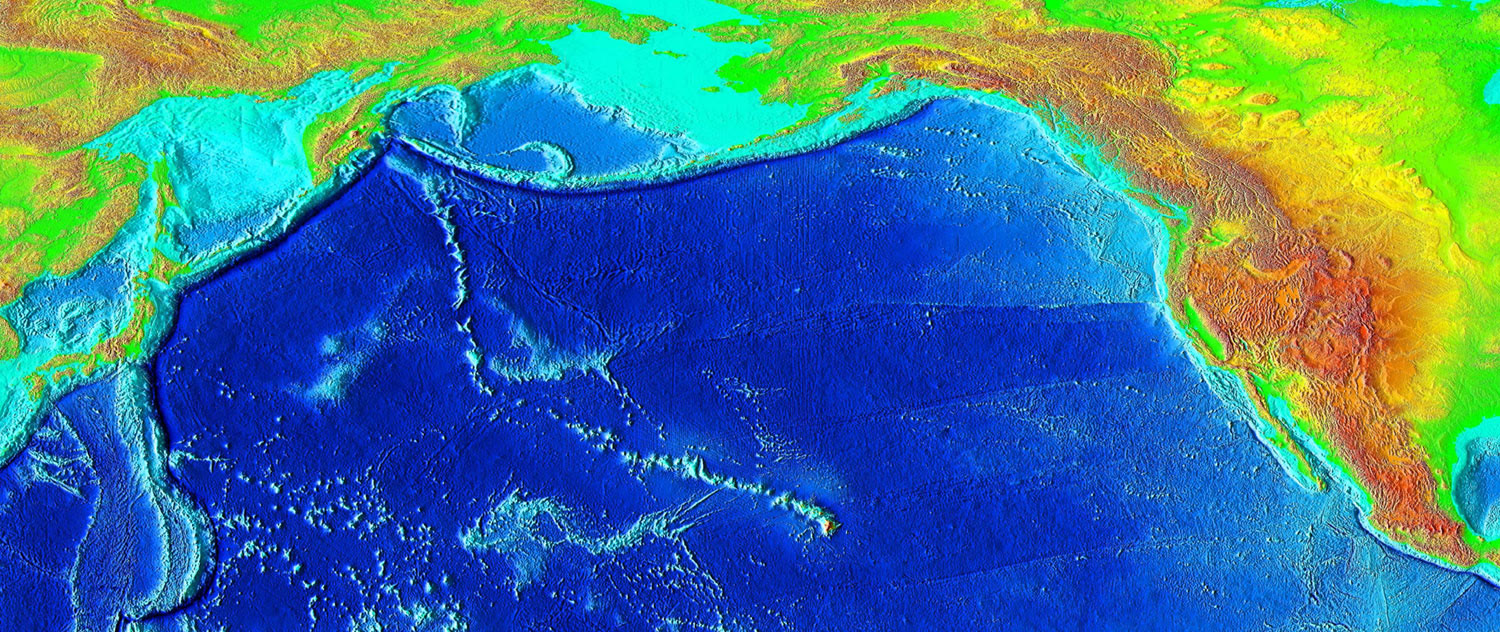
\includegraphics[width=\linewidth]{images/book2/g11-ngdc-hawaii-chain.jpg}

{\small Relieve sombreado del fondo del Pacífico norte. La cadena de Hawái va
desde la isla de Hawái (abajo en el centro, en marrón) hacia el
oeste-noroeste; en el codo gira hacia el norte con los montes submarinos del
Emperador, que terminan en la fosa que bordea Kamchatka y las Aleutianas.
Imagen: National Geophysical Data Center, NOAA (dominio público).}
\end{omfigure}
% ledger: photo:g11-hawaii-chain

La datación potasio--argón de lavas de 37 volcanes de la cadena, recogidas en
las islas, dragadas en los montes submarinos o extraídas por perforación a
través de sus sedimentos, da sus edades (gráfica siguiente). El Mauna Kea
tiene unos \num{0.4} millones de años, Kauai \num{5.1}, Midway \num{27.7} y el
monte submarino Suiko, cerca del extremo de la cadena del Emperador,
\num{64.7}. Las edades crecen con la distancia a Kilauea, el volcán activo,
como predice una \omterm{def:g11:plate-motions:hotspot-track}{traza de punto caliente}.
% ledger: cd87:ages

\begin{omfigure}
\begin{tikzpicture}
\begin{axis}[ompt, width=0.82\linewidth, height=6.4cm, xmin=0, xmax=5000, ymin=0, ymax=70,
  xlabel={distancia a Kilauea a lo largo de la cadena (\unit{km})}, ylabel={edad (millones de años)},
  xticklabel style={/pgf/number format/set thousands separator={}},
  legend style={font=\scriptsize, at={(0.03,0.97)}, anchor=north west}, legend cell align=left]
% computed in figdata/grade-11/hawaii_chain.py; ledger: cd87:ages
\addplot[only marks, mark=o, mark size=1.6pt, omDef, error bars/.cd, y dir=both, y explicit]
  table[x=dist, y=age, y error=err] {figdata/out/grade-11-hawaii_chain-hawaiian.dat};
\addplot[only marks, mark=triangle, mark size=2pt, omProp, error bars/.cd, y dir=both, y explicit]
  table[x=dist, y=age, y error=err] {figdata/out/grade-11-hawaii_chain-emperor.dat};
\addplot[black, densely dashed, line width=0.6pt] table[x=dist, y=age] {figdata/out/grade-11-hawaii_chain-fit.dat};
\legend{cadena de Hawái, codo y cadena del Emperador, {recta por el origen, \qty{9.1}{cm} al año}}
\draw[black!50, densely dotted] (axis cs:3400,0) -- (axis cs:3400,70);
\node[font=\scriptsize, anchor=south, rotate=90] at (axis cs:3400,8) {codo};
\node[font=\scriptsize, anchor=north west] at (axis cs:519,5.1) {Kauai};
\node[font=\scriptsize, anchor=south] at (axis cs:2432,30) {Midway};
\node[font=\scriptsize, anchor=south east] at (axis cs:4860,65.5) {Suiko};
\end{axis}
\end{tikzpicture}

{\small Edad de los volcanes de la cadena Hawái--Emperador frente a su
distancia a Kilauea, con las incertidumbres de las edades. A lo largo de la
cadena de Hawái los puntos siguen una recta que pasa por el origen; más allá
del codo las edades crecen más deprisa con la distancia. Datos: Clague y
Dalrymple (1987).}
\end{omfigure}

A lo largo de la cadena de Hawái, hasta unos \qty{3300}{km}, los puntos se
dispersan alrededor de una recta que pasa por el origen. La recta que mejor
se ajusta a los 26 volcanes datados de esta parte sube un millón de años cada
\qty{91}{km}: según la \cref{prop:g11:plate-motions:hotspot}, la placa del
Pacífico se ha movido sobre el punto caliente a unos \qty{91}{km} por millón
de años, \qty{9.1}{cm} al año. Los autores de las edades, que ajustaron toda
la cadena a su manera, obtuvieron \qty{8.6}{cm} al año.
% ledger: cd87:ages (fit computed in hawaii_chain.py), cd87:rate

Más allá del codo, las edades crecen más deprisa con la distancia: a lo largo
de la cadena del Emperador la placa se movió más despacio, unos
\qty{6.5}{cm} al año de media (mejor recta por los nueve montes submarinos
datados). Y la cadena cambia de dirección. Si el punto caliente no se movió,
el codo registra un cambio en la dirección del movimiento de la placa del
Pacífico. Edades más recientes sitúan el comienzo del codo cerca del monte
submarino Kimmei, hace unos 50 millones de años, al mismo tiempo que una
reorganización de las dorsales del Pacífico y los primeros volcanes de los
arcos insulares de su borde occidental: la placa cambió de rumbo.
% ledger: cd87:ages (Emperor fit computed in hawaii_chain.py), sc06:bend

\section{La capacidad predictiva del modelo}\label{sec:g11:plate-motions:predictive}

El modelo de placas dice que unas pocas \omterm{def:g11:plate-motions:rigid-plate}{placas rígidas} giran alrededor de sus
polos de rotación, y que casi todo ocurre en sus límites. Su fuerza es que
medidas hechas con métodos completamente distintos, a lo largo de lapsos de
tiempo muy diferentes, dan las mismas respuestas.

\begin{itemize}
  \item \emph{Los terremotos y los volcanes} se concentran a lo largo de los
        límites, y el tipo de límite predice su tipo: terremotos someros a lo
        largo de las dorsales, profundos solo cerca de las fosas (el \cref{ch:g11:subduction-zones}).
  \item \emph{El fondo oceánico} es más joven a lo largo de las dorsales y
        cada vez más antiguo al alejarse de ellas, simétricamente a ambos lados
        (el \cref{ch:g11:drift-to-spreading}).
  \item \emph{Las cordilleras} se levantan donde las placas convergen: la
        India sigue avanzando hacia Eurasia a unos \qty{4.5}{cm} al año a
        través del Himalaya, según los polos de rotación (el \cref{ch:g12:mountain-building}).
  \item \emph{Las velocidades concuerdan de un método a otro}: la tabla
        siguiente compara las velocidades medidas hoy por posicionamiento por
        satélite con las que predicen los polos de rotación, cuyas \omterm{def:g11:drift-to-spreading:spreading-rate}{velocidades
        de expansión} proceden sobre todo de las bandas magnéticas y promedian
        el movimiento de los últimos \num{0.8} a \num{3.2} millones de años, y
        con la velocidad que registra una \omterm{def:g11:plate-motions:hotspot-track}{traza de punto caliente} a lo largo
        de decenas de millones de años.
\end{itemize}
% ledger: nnr56:poles, nnr56:data (India-Eurasia computed in plate_velocities.py at 85 E 28 N)

\begin{center}
\small
\begin{tabular}{|l|c|c|}
\hline
qué se mide & método & velocidad (\unit{cm} al año) \\ \hline
Mauna Kea, placa del Pacífico & posicionamiento por satélite, 30 años & 7.2 \\
Mauna Kea, placa del Pacífico & polo de rotación & 6.9 \\
Wettzell, placa euroasiática & posicionamiento por satélite, 31 años & 2.6 \\
Wettzell, placa euroasiática & polo de rotación & 2.3 \\
\shortstack[l]{placa del Pacífico sobre\\el punto caliente de Hawái} & edades de volcanes, 40 millones de años & 9.1 \\ \hline
\end{tabular}
\end{center}
% ledger: data:b2-ngl-gnss, nnr56:poles, cd87:ages (all computed in figdata/grade-11)

Las velocidades de los polos de rotación y las de las estaciones concuerdan
con un margen de \qty{0.3}{cm} al año, aunque las primeras promedian millones
de años y las segundas solo décadas: las placas se mueven hoy como se han
movido durante millones de años. La velocidad del punto caliente es mayor:
se mide en otro marco, el del propio punto caliente, y a lo largo de un
tiempo mucho más largo.

Aparece un rasgo más cuando se comparan las velocidades de placas enteras.
Las placas más rápidas, la de Cocos, la de Nazca, la del Pacífico, la
australiana y la de Filipinas, tienen todas un largo borde que se hunde en el
manto en una fosa; sus velocidades medias rondan de media los
\qty{6.5}{cm} al año. Las placas sin un borde así, entre ellas la
euroasiática, la norteamericana, la sudamericana, la africana y la antártica,
se mueven de media a unos \qty{2.4}{cm} al año. Esta pista sobre lo que mueve
las placas se retoma en el \cref{ch:g11:subduction-zones}.
% ledger: nnr56:rms (means computed in plate_velocities.py)

\section{Ejercicios}

\begin{exercise}[$\star$]\label{exo:g11:plate-motions:1}
Define una \omterm{def:g11:plate-motions:rigid-plate}{placa rígida}. ¿Dónde se concentra la deformación de la \omterm{def:g11:lithosphere-asthenosphere:lithosphere}{litosfera},
y qué observación sísmica cotidiana lo muestra?
\end{exercise}

\begin{exercise}[$\star$]\label{exo:g11:plate-motions:2}
La estación del Mauna Kea se mueve \qty{72}{mm} al año. Expresa esta velocidad
en kilómetros por millón de años. ¿Cuánto se desplaza la estación en 30 años?
¿Y en un millón de años?
\end{exercise}

\begin{exercise}[$\star$]\label{exo:g11:plate-motions:3}
En diez años, una estación se desplazó \qty{30}{cm} hacia el este y
\qty{40}{cm} hacia el norte. Halla sus velocidades hacia el este y hacia el
norte, su velocidad y el ángulo que forma su dirección con el norte.
\end{exercise}

\begin{exercise}[$\star$]\label{exo:g11:plate-motions:4}
Define una \omterm{def:g11:plate-motions:hotspot-track}{traza de punto caliente}. A lo largo de la cadena de Hawái, ¿dónde
está el volcán más joven, y en qué dirección aumentan las edades? ¿Qué indica
eso sobre la dirección en la que se mueve la placa del Pacífico?
\end{exercise}

\begin{exercise}[$\star$]\label{exo:g11:plate-motions:5}
Kauai está a \qty{519}{km} de Kilauea a lo largo de la cadena, y sus lavas más
antiguas tienen \num{5.1} millones de años. Suponiendo que el punto caliente
es fijo, ¿a qué velocidad media lo ha transportado la placa, en kilómetros por
millón de años y en centímetros al año?
\end{exercise}

\begin{exercise}[$\star\star$]\label{exo:g11:plate-motions:6}
En la gráfica de las series de las dos estaciones, la estación de Wettzell se
desplazó unos \qty{63}{cm} hacia el este y \qty{48}{cm} hacia el norte en 31
años. Halla sus velocidades hacia el este y hacia el norte, su velocidad y su
dirección. Compara su velocidad con la del Mauna Kea.
\end{exercise}

\begin{exercise}[$\star\star$]\label{exo:g11:plate-motions:7}
En Islandia, a \ang{64.5} N y \ang{18} O, los polos de rotación dan a la placa
norteamericana la velocidad $(-10.5, +20.6)$ y a la placa euroasiática
$(+7.7, +16.3)$, en milímetros al año (este, norte). (1) Halla la velocidad de
América del Norte respecto de Eurasia, su módulo y su dirección. (2) ¿Qué
representa esta velocidad para la dorsal que atraviesa Islandia? (3) Compárala
con el valor de \qty{2}{cm} al año que se cita a menudo para el Atlántico
Norte.
\end{exercise}

\begin{exercise}[$\star\star$]\label{exo:g11:plate-motions:8}
La placa del Pacífico gira \ang{0.651} por millón de años. (1) Halla la
velocidad de un punto situado a \ang{90} de su polo de rotación, en
centímetros al año. (2) ¿Y la de un punto a \ang{30} del polo? (3) ¿En qué
lugar de una placa es nula la velocidad? ¿Puede darse con un solo número la
velocidad de una placa entera?
\end{exercise}

\begin{exercise}[$\star\star$]\label{exo:g11:plate-motions:9}
Al norte del Himalaya, a \ang{28} N y \ang{85} E, los polos de rotación dan a
la placa india la velocidad $(+40.6, +38.6)$ y a la placa euroasiática
$(+24.0, -3.3)$, en milímetros al año (este, norte). (1) Halla la velocidad de
la India respecto de Eurasia, su módulo y su dirección. (2) Si no cambiara,
¿cuánto convergerían las dos placas en 10 millones de años?
\end{exercise}

\begin{exercise}[$\star\star$]\label{exo:g11:plate-motions:10}
Necker está a \qty{1058}{km} de Kilauea y tiene \num{10.3} millones de años;
Midway está a \qty{2432}{km} y tiene \num{27.7} millones de años. Halla la
velocidad de la placa sobre el punto caliente entre las épocas en que se
formaron los dos volcanes. Compárala con \qty{9.1}{cm} al año.
\end{exercise}

\begin{exercise}[$\star\star$]\label{exo:g11:plate-motions:11}
En un punto, la placa $A$ se mueve \qty{3}{cm} al año hacia el este respecto
de la placa $B$, y la placa $B$ se mueve \qty{4}{cm} al año hacia el norte
respecto de la placa $C$. (1) Dibuja el triángulo de velocidades y halla la
velocidad de $A$ respecto de $C$: módulo y dirección. (2) ¿Cuál es la
velocidad de $C$ respecto de $A$?
\end{exercise}

\begin{exercise}[$\star\star\star$]\label{exo:g11:plate-motions:12}
El Mauna Kea está a \qty{54}{km} de Kilauea y tiene \num{0.375} millones de
años. (1) ¿Qué velocidad da para la placa? (2) Un volcán mide algunas decenas
de kilómetros de ancho, y crece durante varios cientos de miles de años.
Supón que su distancia al punto caliente tiene una incertidumbre de
\qty{25}{km}: ¿entre qué valores está entonces la velocidad? (3) Explica por
qué los volcanes jóvenes cercanos al punto caliente dan una mala estimación de
la velocidad, y por qué los volcanes alejados de él son mejores.
\end{exercise}

\begin{exercise}[$\star\star\star$]\label{exo:g11:plate-motions:13}
Las posiciones mensuales de una estación se dispersan unos \qty{5}{mm}
alrededor de su recta. Un movimiento se ve con claridad cuando supera diez
veces la dispersión. (1) ¿Cuánto tiempo hay que medir para ver con claridad
el movimiento de la estación del Mauna Kea, \qty{72}{mm} al año? (2) ¿Y un
movimiento de \qty{5}{mm} al año, como el que hay a través de una región que
se deforma lentamente en el interior de un continente? (3) ¿Por qué se
midieron las velocidades de las placas con las bandas magnéticas mucho antes
de que los satélites pudieran medirlas?
\end{exercise}

\begin{exercise}[$\star\star\star$]\label{exo:g11:plate-motions:14}
En la dorsal mesoatlántica a \ang{30} S (\ang{13.5} O), los polos de rotación
dan a la placa sudamericana la velocidad $(-4.9, +11.0)$ y a la placa
africana $(+27.1, +17.9)$, en milímetros al año (este, norte).
(1) Halla la velocidad de América del Sur respecto de África, su módulo y su
dirección. (2) Deduce la \omterm{def:g11:drift-to-spreading:spreading-rate}{velocidad de expansión total} y la semivelocidad de
expansión de la dorsal. (3) Los sedimentos del Atlántico Sur dieron una
semivelocidad de unos \qty{1.9}{cm} al año como media de los últimos 66
millones de años (el \cref{ch:g11:drift-to-spreading}). Compara, y propón qué
puede significar la diferencia.
\end{exercise}

\begin{exercise}[$\star\star\star$]\label{exo:g11:plate-motions:15}
Una estación se mueve de forma constante \qty{20}{mm} al año hacia el este.
Justo a mitad de diez años de medidas, un terremoto la desplaza de golpe
\qty{50}{mm} hacia el oeste. (1) Esboza su posición este frente al tiempo.
(2) ¿Qué velocidad se obtendría usando solo la primera y la última posición?
(3) ¿Qué velocidad da cada una de las dos mitades de la serie, por separado?
(4) ¿Cómo debe tratar un geodesta un salto así?
\end{exercise}

\section{Problema: leer la cadena Hawái--Emperador}

\begin{problem}[{Problema de fin de semana --- la velocidad de una placa escrita en volcanes}]
\label{pb:g11:plate-motions:1}
% values from Clague and Dalrymple 1987, Table 1.4 (ledger cd87:ages); fits computed in
% figdata/grade-11/hawaii_chain.py (v_hawaiian 91.2, v_emperor_free 64.6); bend sc06:bend;
% MKEA rates data:b2-ngl-gnss
La tabla da la distancia a Kilauea, medida a lo largo de la cadena, y la edad
potasio--argón de trece volcanes de la cadena Hawái--Emperador. Kilauea es el
volcán activo sobre el punto caliente; el codo está entre Abbott y
Daikakuji.

\begin{center}
\small
\begin{tabular}{|l|c|c||l|c|c|}
\hline
volcán & distancia (\unit{km}) & edad (\unit{Ma}) & volcán & distancia (\unit{km}) & edad (\unit{Ma}) \\ \hline
Mauna Kea & 54 & 0.375 & Abbott & 3280 & 38.7 \\ \hline
Kauai & 519 & 5.1 & Daikakuji & 3493 & 42.4 \\ \hline
Nihoa & 780 & 7.2 & Koko (sur) & 3758 & 48.1 \\ \hline
Necker & 1058 & 10.3 & Ojin & 4102 & 55.2 \\ \hline
Laysan & 1818 & 19.9 & Nintoku & 4452 & 56.2 \\ \hline
Midway & 2432 & 27.7 & Suiko (centro) & 4860 & 64.7 \\ \hline
Colahan & 3128 & 38.6 & & & \\ \hline
\end{tabular}
\end{center}

\medskip
\noindent\textbf{Parte I --- Edades y distancias.}
\begin{enumerate}
  \item ¿Qué volcán de la tabla es el más joven, y cuál el más antiguo? ¿Cómo
        cambian las edades a lo largo de la cadena?
  \item Demuestra que una distancia en kilómetros dividida entre una edad en
        millones de años es una velocidad en milímetros al año.
  \item Calcula la velocidad media $d/t$ que da Kauai.
  \item Calcula $d/t$ para Necker, Laysan, Midway, Colahan y Abbott.
  \item Representa la edad frente a la distancia para los ocho volcanes de la
        tabla situados antes del codo. ¿Quedan los puntos cerca de una recta que pasa por
        el origen?
\end{enumerate}

\medskip
\noindent\textbf{Parte II --- La velocidad de la placa sobre el punto caliente.}
\begin{enumerate}[resume]
  \item Explica por qué, para un punto caliente fijo y una placa que se mueve
        a una velocidad constante $v$, la edad $t$ y la distancia $d$ cumplen $t = d/v$.
  \item Calcula la media de las cinco velocidades de la pregunta~4.
  \item La recta que pasa por el origen y mejor se ajusta a los 26 volcanes
        datados de la cadena de Hawái da \qty{91}{km} por millón de años.
        Compárala con la pregunta~7.
  \item A esta velocidad, ¿cuánto tardaría la placa en llevar Kauai desde el
        punto caliente hasta su posición actual? Compáralo con su edad.
  \item ¿En qué dirección se mueve la placa del Pacífico sobre el punto caliente?
\end{enumerate}

\medskip
\noindent\textbf{Parte III --- El codo.}
\begin{enumerate}[resume]
  \item Calcula la velocidad media de la placa entre las épocas en que se
        formaron Daikakuji y Suiko (centro).
  \item La mejor recta por los nueve volcanes datados desde Daikakuji en
        adelante da \qty{65}{km} por millón de años. Compárala con la
        velocidad a lo largo de la cadena de Hawái.
  \item Edades más recientes sitúan el comienzo del codo cerca del monte
        submarino Kimmei, a \qty{3668}{km} de Kilauea, hace unos 50 millones de años.
        ¿Qué velocidad media da eso para toda la cadena de Hawái?
        Compárala con \qty{91}{km} por millón de años, y explica por qué ambas
        pueden ser correctas.
  \item Si el punto caliente no se movió, ¿qué registra el codo sobre la
        placa del Pacífico?
  \item La datación más reciente encontró grandes cambios de velocidad a lo
        largo de la cadena del Emperador con poco cambio en su dirección.
        Explica por qué la dirección de una cadena y el espaciado de sus edades
        son dos informaciones independientes.
\end{enumerate}

\medskip
\noindent\textbf{Parte IV --- Comparación con la medida actual por satélite.}
\begin{enumerate}[resume]
  \item La estación del Mauna Kea se mueve $\qty{-63.2}{mm}$ al año hacia el
        este y $\qty{+34.5}{mm}$ al año hacia el norte. Halla su velocidad y su
        dirección.
  \item La cadena de Hawái va desde Kilauea hacia el oeste-noroeste. ¿Es
        coherente con ella la dirección de la estación?
  \item La estación da \qty{7.2}{cm} al año; la cadena, \qty{9.1}{cm} al año.
        Da dos razones por las que los dos números no tienen por qué ser iguales.
  \item A \qty{91}{km} por millón de años, ¿cuánto tardará la placa en alejar
        el Mauna Kea otros \qty{100}{km} del punto caliente?
  \item Concluye: ¿a qué velocidad se ha movido la placa del Pacífico sobre el
        punto caliente de Hawái durante los últimos 40 millones de años?
\end{enumerate}
\end{problem}
